\chapter{Observation Methods}\label{ch:obs_methods}

This chapter will describe four methods currently in use for the detection of exoplanets.  While these do not represent all of the ways that have been proposed or successfully employed to study exoplanets, three of these (doppler spectroscopy, transit photometry, and astrometry) have provided us with the bulk of the currently known exoplanets, while direct detection promises to be a very powerful tool for future exoplanet study, and a subject of much interest in the community.  These four methods also fit well into the common parameter set described in \S\ref{sec:exosystem_params}, which makes it simpler to discuss applications incorporating data derived from more than one of these methods.


\section{Direct Detection}\label{sec:direct_detection}

Direct detection (or imaging) instrumentation can be split roughly into two classes: internal coronagraphs and external occulters.  Broadly speaking, internal coronagraphs seek to create regions of high contrast in the image plane by generating specialized PSFs.  This is achieved with various combinations of shaped pupils \citep{vanderbei2004checkerboard, vanderbei2003circularly, kasdin2005}, apodized pupils \citep{jacquinot1964progress, nisenson2001detection}, Lyot stops \citep{kuchner2002coronagraph, soummer2004apodized}, pupil mapping systems \citep{guyon2003,vanderbei2006diffraction}, etc. As these systems are highly sensitive to minute surface errors on any of the optical elements, they often include deformable mirrors (DMs) as part of active wave-front control systems to correct for any errors introduced in the wavefront by internal optics \citep{pueyo2008broadband}.  This adds a great deal of complexity to these systems and requires precise wavefront estimation and broadband wavefront correction, both of which are extremely difficult \citep{groff2010progress}.

\begin{figure}[ht]
 \center
 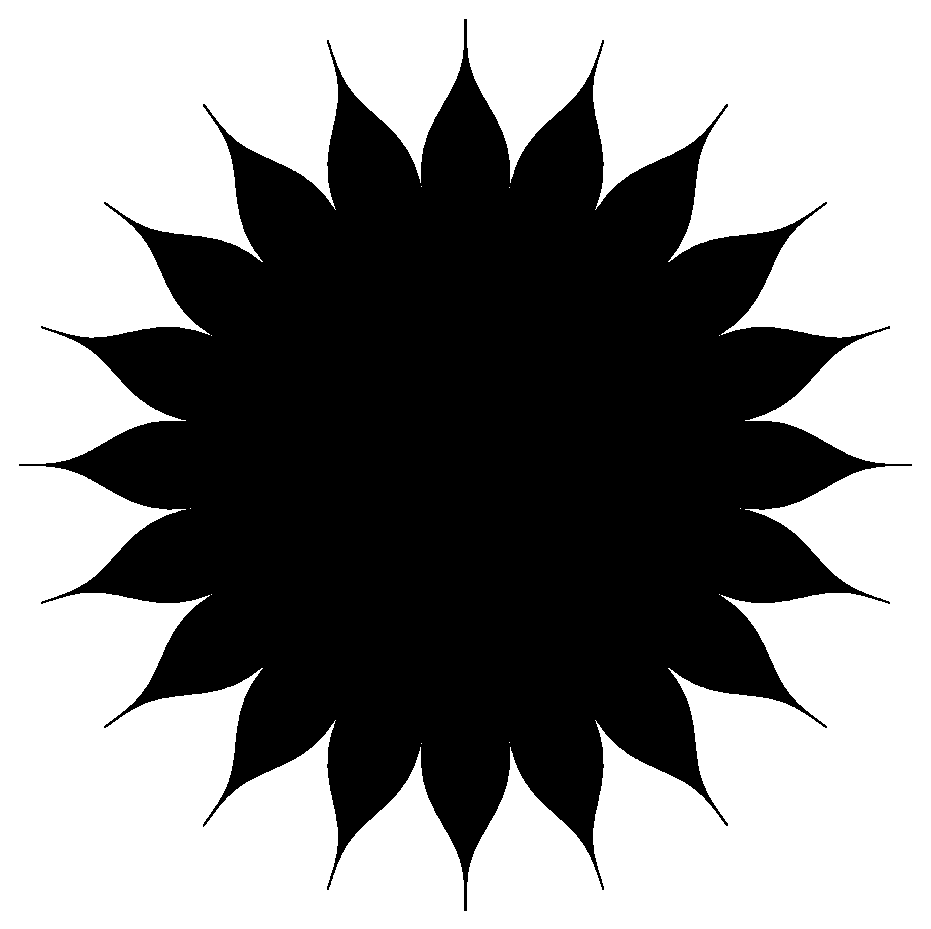
\includegraphics[width=3in]{./figures/theiaOcculter}
  \caption[Starshade]{ \label{fig:theiaOcculter} A starshade.  The `petals' are designed to prevent diffraction of light about the central disk, thereby creating a dark region at the aperture of the telescope.}
 \end{figure}
Alternatively, external coronagraphs use a separate spacecraft (an `occulter' or `starshade'; see \reffig{fig:theiaOcculter}) between the target and the telescope to block most of the starlight from entering the telescope pupil \citep{cash2006detection,vanderbei2007,cady2010design}.  This means that the telescope itself can be fairly conventional, as the contrast level in the image plane no longer needs to be large to detect planets.  This also means that 
active wavefront control is not required, as the system is no longer highly sensitive to small errors in the optical surfaces.  However, the occulter must be flown in exact formation with the telescope throughout observations, at separations of tens of thousands of kilometers and required alignment precisions of tens of centimeters, yielding a very difficult control problem \citep{sirbu2010dynamical}.  The starshade must also be manufactured to very strict tolerances \citep{shaklan2010error}.  The modeling of a direct planetary observation will follow the descriptions in  \citet{brown2005} and \citet{savransky2010}, and will be applicable to both types of imaging systems.  

\subsection{Imaging Observables and Constraints}\label{sec:imag_inst_obs}
An observation of a planet in reflected or emitted light produces two pieces of information: the planet's position and brightness.  In most cases, these values will be relative to the primary star, providing us with the planet's position relative to the star in the plane of the sky (with respect to the observer) and the ratio of fluxes between the planet and star.  This makes it useful to define a `sky' frame,  $\mc S = (S,\mf s_1, \mf s_2, \mf s_3)\addsymbol{$\mc S$}{Sky frame}$ where the the observer line of sight to the target star is along $\mf s_3$, and the plane of the sky (from the viewpoint of the observer) lies in $(\mf s_1, \mf s_2)$.  That is, 
\begin{equation}
\frac{\mf r_{S/sc}}{\Vert \mf r_{S/sc}\Vert} \equiv \mf s_3 \,,
\end{equation}
as shown in Figure \ref{fig:orbit_diagram}.  In contrast to \refeq{eq:rpsP1}, we begin with the planar orbit orientation in $(\mf s_2, \mf s_3)$:
\begin{equation}
[\mf r_{P/S}]_{\mc P} = \left[ \begin{matrix} 0 \\ r\sin\nu \\r\cos\nu \end{matrix}\right] \,.
\end{equation}
Since the 3-1-3 rotation can orient the orbit in all directions throughout the unit sphere, the initial orientation can be in any plane.  The $(\mf s_2, \mf s_3)$ plane is used here to conform to earlier studies and allow simpler comparison of the results.  Following \refeq{eq:rpsrot}, we use the Euler angle set $(\psi,\theta,\phi)_{\mc S}$ to write:
\begin{equation}\label{eq:rpsdef}
[\mf r_{P/S}]_{\mc S}
= \left[
\begin{array}{c} r (\cos\nu  \sin\theta  \sin\phi +\sin\nu  (\cos\theta  \cos\psi  \sin\phi +\cos\phi
 \sin\psi )) \\
 r (\cos\nu  \cos\phi  \sin\theta +\sin\nu  (\cos\theta  \cos\phi  \cos\psi -\sin\phi
 \sin\psi )) \\
 r (\cos\theta  \cos\nu -\cos\psi  \sin\theta  \sin\nu )
\end{array}
\right] \,.
\end{equation}

\begin{figure}[ht]
 \center
 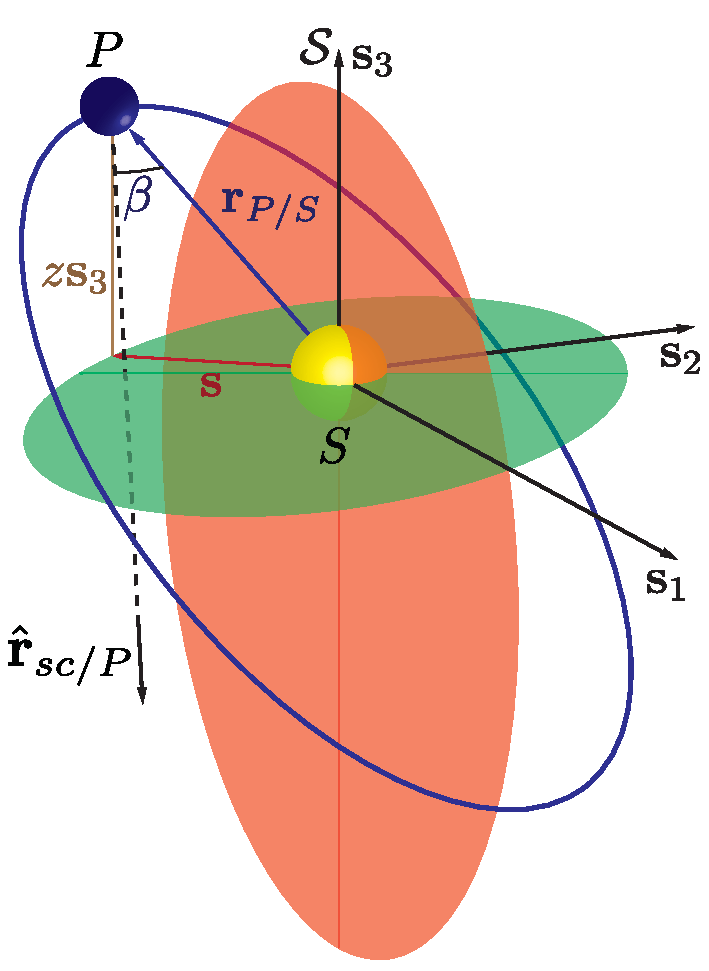
\includegraphics[width=3in]{./figures/orbit_diagram}
  \caption[Orbit Diagram]{ \label{fig:orbit_diagram} Schematic of a planetary orbit.  The green shaded ellipse represents the projection of the orbit into the plane of the sky ($\mf s_1$, $\mf s_2$), while the red shaded ellipse represents the planar orbit in ($\mf s_2$, $\mf s_3$).}
 \end{figure}
We define the separation $\mf s \addsymbol{$\mf s$}{Sky star-planet vector}$ as the projection of the star-planet vector into the plane of the sky:
\begin{equation}\label{eq:svdef}
[\mf s]_{\mc S} = \left[\begin{array}{ccc}1 & 0 & 0 \\ 0 & 1 & 0 \\ 0 & 0 & 0\end{array}\right] [\R_{p/s}]_{\mc S} \, ,
\end{equation}
as in Figure \ref{fig:orbit_diagram}.   This projection also leads us to define the apparent separation - the magnitude of the star-planet vector projected into the plane of the sky:
\begin{equation}\label{eq:sdef} \addsymbol{$s$}{Apparent separation} 
s = \Vert \mf s \Vert \,.
\end{equation}
The apparent separation may be either a derived quantity (when the instrument is capable of resolving the star-planet separation in two dimensions, or can measure the absolute planet position with respect to another reference like the solar system barycenter) or a primary observable (when the instrument can only measure the separation in one dimension).

The relative flux between the planet and its parent star is a function of the orbital radius and the planet's albedo and radius:
\begin{equation} \label{eq:fluxRatiodef}  \addsymbol{$F_R$}{Ratio of planet to star fluxes}
F_R \triangleq \frac{F_p}{F_s} = p\Phi(\beta) \left(\frac{R}{r}\right)^2 \, ,
\end{equation}
where $\Phi\addsymbol{$\Phi$}{Planet phase function}$  is the planet's phase function \citep{sobolev}, and $\beta\addsymbol{$\beta$}{Phase angle}$  is the star-planet-observer (phase) angle, given by:
\begin{equation}  
\beta = \cos^{-1}\left(\frac{\mf r_{P/sc} \cdot  \mf r_{P/S} }{\Vert \mf r_{P/sc} \Vert  \Vert\mf r_{P/S}\Vert}\right) \, ,
\end{equation}
where $\R_{P/sc}$ is the position of the planet relative to the observer:
\begin{equation}
\Vert \mf r_{P/sc} - \mf r_{sc/O} - \mf r_{P/S}\Vert = d \, .
\end{equation}
However, since $d \gg r $, we can make the approximation:
\begin{equation}  \label{eq:betadef}
\beta \approx \cos^{-1}\left(\frac{z}{r}\right) \, .
\end{equation}
where $z$ is the $\mf s_3$ axis component of $[\mf r_{p/s}]_{\mc S}$.  For the closest star to Earth (approximately 1.3 pc away), this approximation produces errors of less than 0.001\%.  The flux ratio is often expressed on a logarithmic scale, in which case it becomes the difference in magnitude between the star and planet:
\begin{equation}\label{eq:deltamagdef} \addsymbol{$\Delta$mag}{Difference in magnitude between star and planet}
\Delta\textrm{mag} \triangleq -2.5\log_{10}F_R \,.
\end{equation}

Observable limits on $s$ and $F_R$, or functions thereof, can be mapped to instrument specifications for a fairly broad variety of direct imaging instruments by assuming that a planet will be observable if its angular separation from the star is greater than the observatory's inner working angle (IWA)$\addsymbol{IWA}{Inner working angle}$, and illuminated such that the $\Delta$mag is below a threshold value, called the limiting $\Delta$mag, or $\Delta$mag$_0\addsymbol{$\Delta$mag$_0$}{Limiting $\Delta$mag}$.  The IWA represents the minimum angular separation between the telescope's central axis (line of sight) and detectable objects on the sky.  The specific determination of the IWA depends on the instrument design, and may be affected by the size of a central obscuration, the capability of an adaptive optics systems to remove light from certain areas of the image plane, or the size and geometry of external occulting optics.  

The limiting $\Delta$mag represents the point where systematic errors produce unresolvable confusion between planet signal and background noise \citep{brown2005}.   It is important to note that while this value is often equated with the designed contrast of an instrument (i.e., the ratio of the core to halo of a coronagraph's point spread function), they are not necessarily the same.  Depending on the nature of the background and instrument systematics, $\Delta$mag$_0$ may actually be less than the designed contrast.  In fact, it is becoming standard practice to set the design contrast at several magnitudes below the $\Delta$mag$_0$ required by the population of interest, based on a detailed error budget (see, for example, \citet{shaklan2010error}).  \reffig{fig:imagingConstraintsSchem} shows a schematic of the instrument constraints on direct imaging.
\begin{figure}[ht]
 \center
 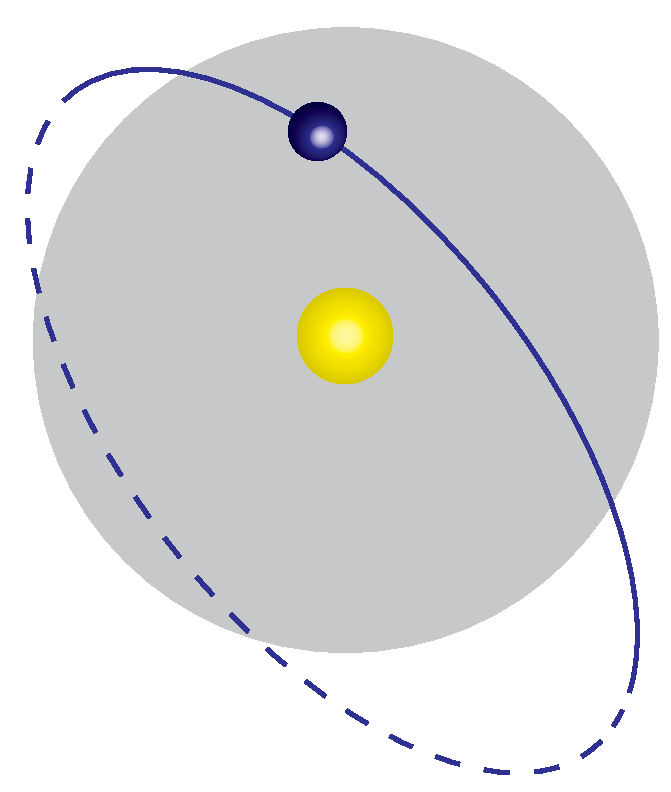
\includegraphics[width=3in]{./figures/imagingConstraintsSchem}
  \caption[Imaging constraints diagram]{ \label{fig:imagingConstraintsSchem} Schematic of the instrument constraints on direct imaging.  The shaded circle centered on the star represents the projected IWA (no observations can be made within this angle of the star) and the planet is sufficiently illuminated ($\Delta$mag  < $\Delta$mag$_0$) on the solid portion of the orbit (when the planet is between the observer and the star along the line of sight).  In this case, the planet is only observable on two small portions of its orbit near periapsis and apoapsis.}
 \end{figure}

A significant difference between occulters and coronagraphs is the dependence of their IWA on wavelength.  The extent of the coronagraph's produced region of high contrast depends completely on the geometry of the internal optics.  If the region extends to some location $n$ in the image plane, then it represents an aperture plane location of $n/f \lambda/D$ where $D$ is the aperture diameter and $f$ is the focal length.  Thus, the IWA for the coronagraph is commonly given in units of $\lambda/D$, and changes with wavelength.  An occulter, on the other hand creates a region of high contrast over a specific wavelength band.  In this case, the light from the star is removed before it ever gets to the telescope, so the dark region extends throughout the entire image plane.  On the other hand, if the angular separation of the planet from the star is less than the angular size of the occulter on the sky, then the light from the planet will also be blocked.  Therefore, the IWA (often called the geometric IWA) for the occulter is set by its radius $R_O$ and separation distance from the telescope $d_s\addsymbol{$d_s$}{Occulter separation distance}$:
\begin{equation}
\textrm{IWA}_\textrm{geom} = \sin^{-1}\left(\frac{R_O}{d_s}\right) \,.
\end{equation}
Because occulters are designed with petals (as in \reffig{fig:theiaOcculter}), it is actually possible to see some of the planet light coming through the gaps between the petals when the planet is inside the geometric IWA, albeit at a significantly decreased system throughput.

\begin{figure}[ht]
 \center
 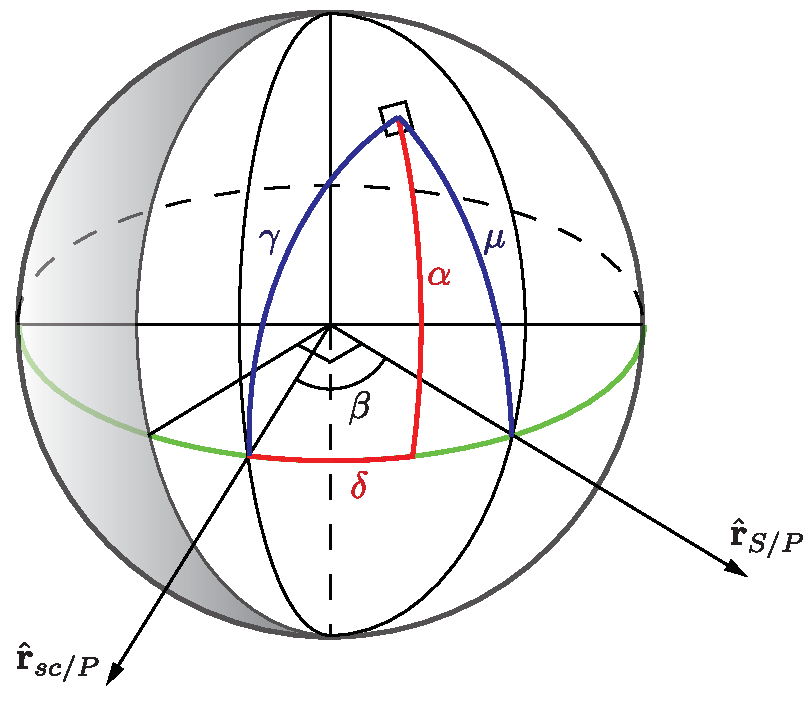
\includegraphics[width=4in]{./figures/reflection_diagram}
  \caption[Reflection Diagram]{ \label{fig:reflection_diagram} Schematic of a reflecting spherical body.  The angles $(\alpha, \delta)$ are the coordinates of an arbitrary point on the surface, $\mu$ is the angle of incident radiation, and $\gamma$ is the angle of emergent radiation.}
 \end{figure}
 We have so far defined all of the elements that are used to calculated $s$ and $F_R$, except for the phase function.  Unfortunately, there can be no single definition for $\Phi$, as it depends on the characteristics of a given planet.  One way to get around this difficulty is to assume that the planet can be modeled as a Lambertian reflector, i.e., that the planet's surface luminance is isotropic.  This leads to the commonly used Lambert phase function.  Because of the importance of this function, it is useful to briefly derive it here.  Following \citet{sobolev}, we let $(\alpha, \delta)$ be the planetary latitude and longitude of an arbitrary point on the planet's surface, $\mu$ the angle of incident radiation, $\gamma$ the angle of emergent radiation at a surface point, and $\xi$ the azimuthal angle between $\mu$ and $\gamma$ such that:
\begin{equation}
\cos \xi = \frac{\cos\mu\cos\gamma - \cos\beta}{\sin\mu\sin\gamma} \,.
\end{equation}
These definitions are shown schematically in \reffig{fig:reflection_diagram} and yield the realtionships:
\begin{align}
	\cos\mu &= \cos\alpha \cos(\beta - \delta) \triangleq C_\mu \,,\\
	\cos\gamma &= \cos\alpha \cos\delta \triangleq C_\gamma \,.
\end{align}
	
The emergent intensity is given by:
\begin{equation}
I = C_\gamma F \rho(C_\mu,C_\gamma,\xi) \,,
\end{equation}
where $\pi C_\gamma F$ is the flux on a patch of the surface and $\rho$ is the reflection coefficient.  The energy crossing a surface patch into unit solid angle is $C_\gamma C_\mu F \rho \intd{A}$ where
\begin{equation}
\mathrm{d}A = R^2 \cos\alpha \intd{\alpha} \intd{\delta} \,.
\end{equation}
The energy per second per unit area per unit solid angle received by an observer is thus:
\begin{equation}
E(\beta) = \frac{F R^2}{r^2} \int_{\beta - \pi/2}^{\pi/2} \cos(\beta - \delta) \cos\delta \intd{\delta}  \int_{-\pi/2}^{\pi/2} \rho(C_\mu,C_\gamma,\xi) \cos^3 \alpha \intd{\alpha}
\end{equation}
The phase function is defined as the ratio of $E(\beta)/E(0)$.  For isotropic scattering, $\rho$ is constant so:
\begin{equation}\label{eq:lambertPhaseFunc}
\Phi_L(\beta) = \frac{\int_{\beta - \pi/2}^{\pi/2} \cos(\beta - \delta) \cos\delta \intd{\delta}}{ \int_{-\pi/2}^{\pi/2} \cos(-\delta) \cos\delta \intd{\delta}} = \frac{\sin(\beta)+(\pi-\beta)\cos(\beta)}{\pi}
\end{equation}

\begin{figure}[ht]
 \center
 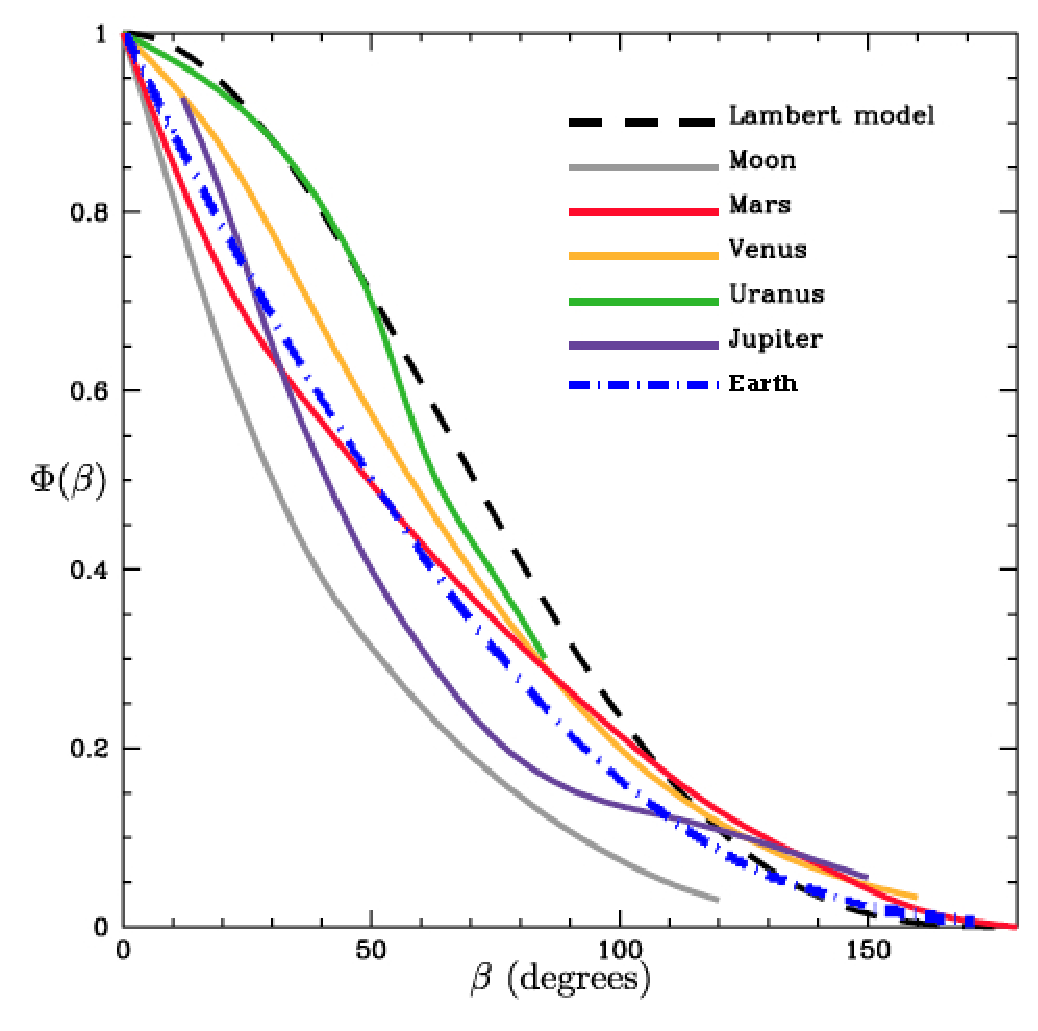
\includegraphics[width=4.5in]{./figures/phi_v_beta}
  \caption[Solar system planet phase functions]{ \label{fig:phi_v_beta} Empirically determined phase functions of solar system bodies plotted with the Lambert phase function.  Data from \citet{sudarsky2005} and \citet{devaucouleurs1964geometric}.}
 \end{figure}
Figure \ref{fig:phi_v_beta} compares the Lambert phase function with empirical values found for the various planetary bodies in the solar system.  It is immediately evident that the assumption of isotropic scattering is not a good one for most of these, as it overestimates the true phase function in almost all cases.  More precise modeling can be achieved by using empirically derived lookup tables, whenever possible.

Having a functional form for the phase function does have certain advantages, however.  For example, we can quantify the relationships between the direct detection observables such as the extrema in planet to star flux ratios as functions of the apparent separation.  By \refeq{eq:betadef}, we can also write:
\begin{equation}
\beta = \sin^{-1}\left(\frac{s}{r}\right)  \quad \Rightarrow \quad r = \frac{s}{\sin\beta} \,,
\end{equation}
so that \refeq{eq:fluxRatiodef}, assuming $\Phi = \Phi_L$, becomes:
\begin{equation}
F_R = \frac{p R^2}{s^2} \sin^{2}\beta\left[ \left( \pi - \beta\right)\cos\beta + \sin\beta \right] \,.
\end{equation}
Following \citet{brown2005}, we differentiate with respect to $\beta$ to find that the extrema of $F_R$ for fixed $p, R$, and $s$ occur when:
\begin{equation}\label{eq:FRminimization}
\sin\beta \left[ \left( \pi - \beta\right)\left( 1+ 3\cos 2\beta \right)+ 2 \sin 2\beta \right] = 0 \,.
\end{equation}
We can thus write the maximum flux ratio as:
\begin{equation}\label{eq:maxFr}
\max F_R =  \frac{p R^2}{s^2} \Phi_L(\beta^\star)
\end{equation}
where $\beta^\star$ is the solution to \refeq{eq:FRminimization} and is approximately equal to 1.1047 rad (63.296$^\circ$).  The other two extrema of $F_R$ given by \refeq{eq:FRminimization} are at $\beta = 0$ and $\beta = \pi$, corresponding to the planet directly in front or behind the star along the observer's line of sight.  As this does not occur for all orbital orientations, it is useful to consider the case of the minimum apparent separation (the planet's closest approach to the star in the plane of the sky) when the planet is between the star and the observer.  This occurs when:
\begin{equation}
\beta =  \pi - \sin^{-1}\left(\frac{s}{r_a}\right) \,,
\end{equation}
where $r_a$ is the orbital radius at  apoapsis, given (for a Keplerian orbit) by $r_a = a(1+e)$.  The minimum flux ratio is thus:
\begin{equation}\label{eq:minFr}
\min F_R =  \frac{p R^2}{r_a^3} \left[s - \sqrt{r_a^2 - s^2}\sin^{-1}\left(\frac{s}{r_a}\right)\right]\,.
\end{equation}
These limits are useful in determining whether an observation belongs to a specific population of planets, or when bounding the expected performance of an instrument (see \S\ref{sec:completeness_apps}).

\subsection{Observation Modeling}\label{sec:model_obs}
When using a direct detection system, an observation of (or `visit' to) a target system can be broken down into two main activities: first, it is necessary to determine whether a planet has been detected; second, in the event of a detection, the planet may be characterized using the specific capabilities of the instrument, which may cover various wavelength ranges with varying spectral resolutions.  Orbital characterization can only be obtained as a result of multiple detections of the same planet and depends on the spatial resolution of the instrument and the ability to accurately centroid in the produced data.  We can model the success or failure of both these tasks based on the time required compared with the time available.

Every visit results in one of four possible outcomes:  detection, missed detection, null detection or false alarm.  A null detection occurs when there are no observable planets at the time of observation.  A missed detection signifies that an observable planet does exist, but was not found (i.e., if the integration time was insufficient to achieve a detection).  On the other hand, a false alarm means that a detection is assumed when there is actually no corresponding planet in the target system (i.e., when noise or other objects in the field of view are mistaken for a planet).  In the case of false alarms, it is assumed that followup spectroscopy will be able to resolve these as null detections (at the cost of additional integration time). In statistical terms, a null detection is a true negative, a missed detection is a false negative, a false alarm is a false positive, and a detection is a true positive.

Following \citet{kasdin2006}, we assume that the instrument produces images with sufficient sampling so that matched filtering (or some other probabilistic detection algorithm) can be applied, which significantly reduces the integration time required to decide whether a planet is present in the field of view.  We treat the photons received at pixel $j$ of the detector array as a random variable of the form
\begin{equation}
z_j = C_p \bar{P}_j + C_b  + \nu
\end{equation}
where $C_p\addsymbol{$C_p$}{Mean photon count at pixel centered on planet PSF}$ and $C_b\addsymbol{$C_b$}{Mean background photon count}$ are the mean photon count at the pixel centered on the point spread function (PSF) and mean background photon count at all pixels, respectively, $\bar{P}$ is the normalized, non-dimensionalized PSF, and $\nu$  is the photon and readout noise.  This allows us to construct a signal to noise metric as the random  variable $\hat{C}_p/\sigma_b$ where $\hat{C}_p$ is the linear, unbiased estimate of the planet signal, and $\sigma_b$ is the variance of this estimate for pixels without a planet.  The assumption made in this metric is that the background contribution is known, or can be estimated during the integration.  We define the ratio of planet to background counts as the parameter $Q\addsymbol{$Q$}{Ratio of planet to background photon counts}$:
\begin{equation}\label{eq:Qdef}
Q \triangleq \frac{C_p}{C_b} \,.
\end{equation}

Simplifying the statistics by assuming the photon arrival rate can be approximated as a Gaussian distribution,  and noting that both $C_p$ and $C_b$ are linear in integration time ($t$), we can write an expression for $t$ based on a desired false alarm probability (FAP$\addsymbol{FAP}{False Alarm Probability}$) and missed detection probability (MDP $\addsymbol{MDP}{Missed Detection Probability}$).  \citet{kasdin2006} derive this expression as:
\begin{equation}\label{eq:detIntTime}
t = \frac{1}{b} \frac{(K - \gamma \sqrt{1 + \tilde{Q} \Xi/\Psi})^2}{\tilde{Q}T_A \Psi}\,,
\end{equation}
where $\tilde{Q}$ is equal to $Q$ scaled by the sum of $\bar{P}$,  
\begin{equation}
\Xi = \frac{\sum_j \bar{P}^3_j}{(\sum_j \bar{P}_j)^3} \,, \quad \textrm{and} \quad
\Psi = \frac{\sum_j \bar{P}^2_j}{(\sum_j \bar{P}_j)^2} \,.
\end{equation}
This last parameter, $\Psi\addsymbol{$\Psi$}{Sharpness}$, is often referred to as the telescope `sharpness'.  The threshold value $K$ is  determined by the required FAP, such that:
\begin{equation}
\Phi(K) = 1 - \textrm{FAP} \,,
\end{equation}
where $\Phi(\cdot)$ represents the Gaussian distribution function.  Similarly, $\gamma$ is the threshold determined by the required MDP, such that:
\begin{equation}
\Phi(\gamma) = \textrm{MDP} \,.
\end{equation}
The final two parameters, $T_A$ and $b$, are derived from properties of the optical system and target star.   The `Airy Throughput', $T_A$, is the starlight suppression system throughput ($T$) multiplied by the non-dimensionalized pixel area and the sum of the normalized PSF \citep{vanderbei2003circularly}.  The parameter $b$ is defined as:
\begin{equation}
b \triangleq \textrm{QE} \, \upsilon I_p(\lambda_r) \Delta \lambda A
\end{equation}
where QE$\addsymbol{QE}{Quantum efficiency}$ is the detector's quantum efficiency, $\upsilon$ is the attenuation of optical elements up to the exit pupil, and $A$ is the entrance aperture area.  The term $I_p(\lambda_r) \Delta \lambda$ represents the total irradiance of the planet in the detection band (centered at $\lambda_r$ with bandwidth $\Delta \lambda$). $I_p(\lambda_r)$ is the average irradiance in this band, and is calculated as
\begin{equation}
I_p(\lambda_r) = \mathcal{F}_010^{-(V_s + \Delta\textrm{mag})/2.5}
\end{equation}
where $V_s$ is the target star's apparent magnitude in the detection band and $\mathcal{F}_0$ is the band specific flux for a zero magnitude star (see \reftable{table:zeroMagFluxes}). 
\begin{table}[ht]
\caption[Zero Magnitude Flux Points]{Zero Magnitude Flux Points. Data from  \citet{colina1996}\label{table:zeroMagFluxes}}
\begin{center}
\begin{tabular}{ c c c c }
\hline\hline
&  Central & & $\mathcal{F}_0$ \\
Filter & Wavelength (nm) & FWHM (nm) & (photons cm$^{-2}$ nm$^{-1}$ s$^{-1}$)\\
\hline
U & 373.5 & 48.5 & 8160.25\\
V & 444.3 & 83.1 & 14314.61\\
B & 548.3 & 82.7 & 9798.73\\
R & 685.5 & 174.2 & 6625.70\\
I & 863.7 & 197.0 & 4082.74\\    
\hline
\end{tabular}
\end{center}
\end{table}
Alternatively, if a model spectrum is available for the target star, this term can be replaced by the integral of the spectrum over $\Delta \lambda$.

Because the basic detection approach used here is one of Bayesian signal processing, the sampling of the image plane has a large effect on the required integration time.  In particular, it is important to have a sufficiently small pixel size, and to use a large enough portion of the PSF in the signal analysis. \reffig{fig:intTimevPSF} shows the normalized integration times for constant values of $b$ and $T$ as a function of size of the PSF used and the pixel area for an open circular aperture.  We see that there exist critical values for each of these beyond which the integration time is nearly constant.  In fact, as long as at least 1.5 $\lambda/D$ of the PSF are sampled, changes in integration time due to different pixel sizes are relatively minor.  The same effect is found when considering non-Airy PSFs.
\begin{figure}[ht]
 \center
 \includegraphics[width=5in]{./figures/intTimevPSF}
  \caption[Integration time vs.~PSF sampling ]{ \label{fig:intTimevPSF} Normalized integration time ($\beta T t$) as a function of half size PSF used and pixel area for an open circular aperture.  The color bar is log-scale, in powers of 10.  Note that insufficient sampling of the PSF can significantly increase the required integration time.}
\end{figure} 

To calculate the value of $Q$ (defined in \refeq{eq:Qdef}) we first define the value:
\begin{equation}
c_1 \triangleq  \textrm{QE} \, \upsilon \Delta\lambda A T t \,.
\end{equation}
This allows us to write:
\begin{equation}\label{eq:Cpdef}
C_p = \mathcal{F}_0 10^{-(V_s + \Delta\textrm{mag})/2.5} c_1 \,,
\end{equation}
and
\begin{equation}\label{eq:Cbdef}
\begin{split}
C_b = &\mathcal{F}_0 10^{-\Omega_{zodi}/2.5} \left(f(\bar{\beta}) +\mu f(I)2.5^{4.78 - M_V} \right) \Delta \alpha c_1\\
&{}+\mathcal{F}_0 10^{-V_s/2.5} C c_1 + \textrm{DR} t + \frac{\sigma_r^2}{t_r}t \,,
\end{split}
\end{equation}
where $C$ is the instrument's designed contrast,  $\Omega_{zodi}$ is the detection band intensity of local zodiacal light in magnitudes per square arcsecond at the ecliptic pole (nominally,  23.34 for V band), $M_V\addsymbol{$M_V$}{Absolute magnitude (V band)}$ is the absolute magnitude of the target star, $\mu\addsymbol{$\mu$}{Brightness of exo-zodi}$ is the brightness of the extrasolar zodiacal light (exo-zodi) in units of local zodi, $\sigma_r$ is the detector read noise, $t_r$ is the exposure time per readout, DR is the detector dark current rate per pixel, and $\Delta\alpha$ is the pixel area on the sky in square arcseconds.  The pixel area can be written as:
\begin{equation}
\Delta \alpha =\Omega\left(\frac{180*3600}{\pi}\right)^2 \,,
\end{equation}
where $\Omega$ is the solid angle of a detector pixel in steradians and equals $(\lambda/2D)^2$ for critically sampled systems with circular apertures \citep{brown2005}.  The function $f$ is the empirically derived variation of zodiacal light with viewing angle given by:
\begin{equation}
f(\theta) = 2.44 - 0.0403 \theta + 0.000269 \theta^2
\end{equation}
with $\theta$ in degrees, in the range [0,90] (the relation is mirrored for $\theta \in (90,180]$).  The function is applied to $\bar{\beta}$ - the absolute value of the ecliptic latitude of the target star, and $I$ - the target star system's inclination\footnote{For mult-planet systems, this refers to the inclination of the ecliptic plane.}(D. Lindler,  Personal Communication, 2008). 

It should be noted that a major assumption being made here is that the exo-zodi is uniform and of constant magnitude in the region being observed.  Recent results indicate that this is not an ideal assumption as exozodiacal dust will clump due to the gravitational effects of any planets and will always have color and brightness variations \citep{kuchner2010collisional}.  If we do select a single value for exo-zodi brightness, then it makes sense to use the historical average for our own solar system.  Based on measurements of seafloor sediment isotope concentrations, the historical distribution of zodical dust in the solar system (over the last 80 Myr) is roughly log normal, with a mean of 1.55 zodi (\reffig{fig:zodi_dist}).  It is predicted that 95\% of solar analogs will have zodiacal dust levels in the range of 0.7 to 3.3 zodi, under the assumption that their asteroid and comet populations are similar to those of our solar system \citep{kuchner2008}.
\begin{figure}[ht]
 \begin{center}
   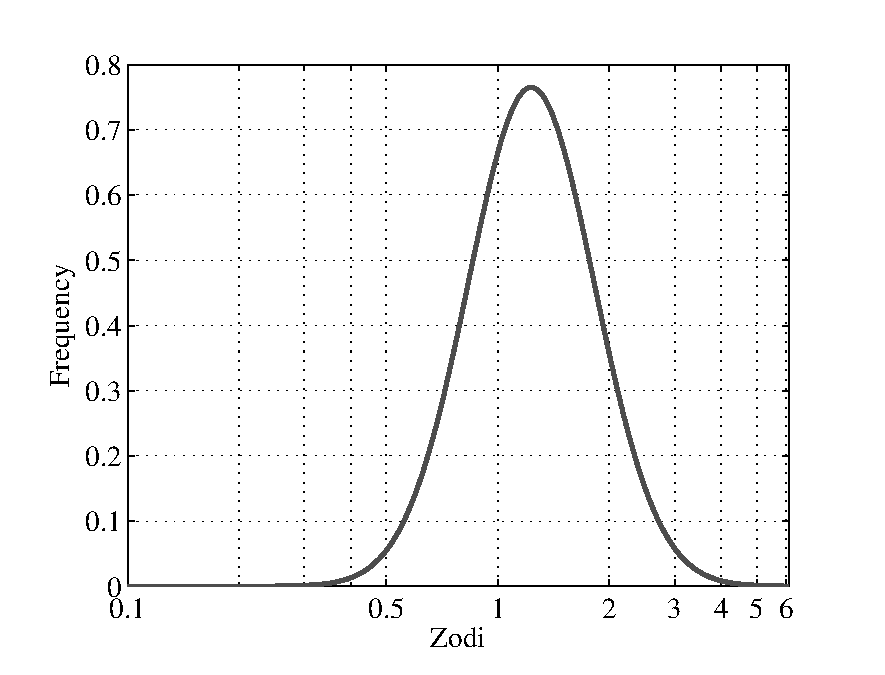
\includegraphics[width=4.5in,clip=true,trim=0.2in 0in 0.5in 0in]{./figures/zodi_dist}
 \end{center}
 \caption[Historical distribution of solar system zodi]{ \label{fig:zodi_dist} Historical distribution of solar system zodiacal dust levels. The distribution is log-normal with geometric mean of 1.55 \citep{kuchner2008}.}
 \end{figure}

Returning to Equations (\ref{eq:Cpdef}) and (\ref{eq:Cbdef}) we evaluate $Q$ as:
\begin{equation}
\begin{split}
Q = \left[\vphantom{\frac{\sigma_r^2}{t_r}} 10^{\Delta\textrm{mag}/2.5} C  + 10^{(V_s +\Delta\textrm{mag}-\Omega_{zodi})/2.5} Z \Delta\alpha \right.
\\
\left. {} + \frac{ 10^{(V_s + \Delta\textrm{mag})/2.5} }{\mathcal{F}_0 \textrm{QE} \, \upsilon \Delta\lambda A T}\left(\textrm{DR} + \frac{\sigma_r^2}{t_r}\right) \right]^{-1} \,,
\end{split}
\end{equation}
 where 
 \begin{equation}
Z = \left(f(\bar{\beta}) +\mu f(I)2.5^{4.78 - M_V} \right)\,.
\end{equation}
In the event of a detection, we calculate the time required for spectral characterization, assuming that the detection integration provides us the magnitude of all background sources.  

Following \citep{lindler2007}, we will represent spectral characterization requirements as minimum signal to noise (S/N$\addsymbol{S/N}{Signal to noise ratio}$) values, using the metric
\begin{equation}
\textrm{S/N} = \frac{C_p}{\sqrt{V}}
\end{equation}
where $V$ is the total variance due to all noise sources.  This value can be written as a function of the square root of the integration time as
\begin{equation}
\textrm{S/N} = \frac{\tilde{C_p} \sqrt{t}}{N_{pix}\left( \left(\frac{\sigma_r^2}{t_r} + \textrm{DR} \right) \left(1 + \frac{1}{N_{dark}}\right) + \mathcal{F}_0 10^{-\Omega_{zodi}/2.5} Z \Delta\alpha \right) + \tilde{C}_p + \tilde{C}_s }
\end{equation}
where $\tilde{C}_p$ and $\tilde{C}_s$ are the planet and star counts per unit time, $N_{dark}$ is the number of dark frames used, and $N_{pix}$ is the number of pixels in the detection box\footnote{This value is often set to the reciprocal of the sharpness (i.e., $N_{pix} = \Psi^{-1}$) \citep{lindler2007}.}.  

The specific S/N value used depends on the spectral feature of interest.  For terrestrial planets, we are especially interested in the possible discovery of biomarkers such as oxygen or ozone.  Several of these features are identified in \citet{heap2007}, along with their S/N requirements; for example, a S/N of 11 for a resolving power of $R = 70$ will produce detections of oxygen at Earth atmospheric levels (21\% ) via the feature at 760nm with a confidence level of over 99.9999\%.  For 20\% Earth O$_2$ abundance, the same signal to noise will still give confidence levels of over 99\% \citep{desmarais2002}.

\section{Astrometry and Doppler Spectroscopy}\label{sec:RV}
While astrometry and doppler spectroscopy employ different technologies and methods to detect planets, they share one thing in common:  namely, these methods infer the presence of planets by tracking the effects of gravitational interactions on the motions of the stars (known as the `astrometric wobble').  The data collected by doppler spectroscopy describes the motion of the target star along the line of sight (the radial velocity), while the data collected by precision astrometry tracks the star's position in the plane of the sky.  Both of these methods therefore require enough observations to fit planetary orbits, which means that the required observing time for confirmed discoveries is directly proportional to the period of planets discovered.  For this reason, there is a strong bias towards short period planets in the early radial velocity data sets \citep{butler2006,cumming2003,cumming2008}.  Similarly, since more massive planets exert a greater effect on their parent stars, these methods are also biased towards larger planets. 

\subsection{Astrometric Observables and Constraints}\label{sec:ast_inst_obs}
\begin{figure}[ht]
\centering
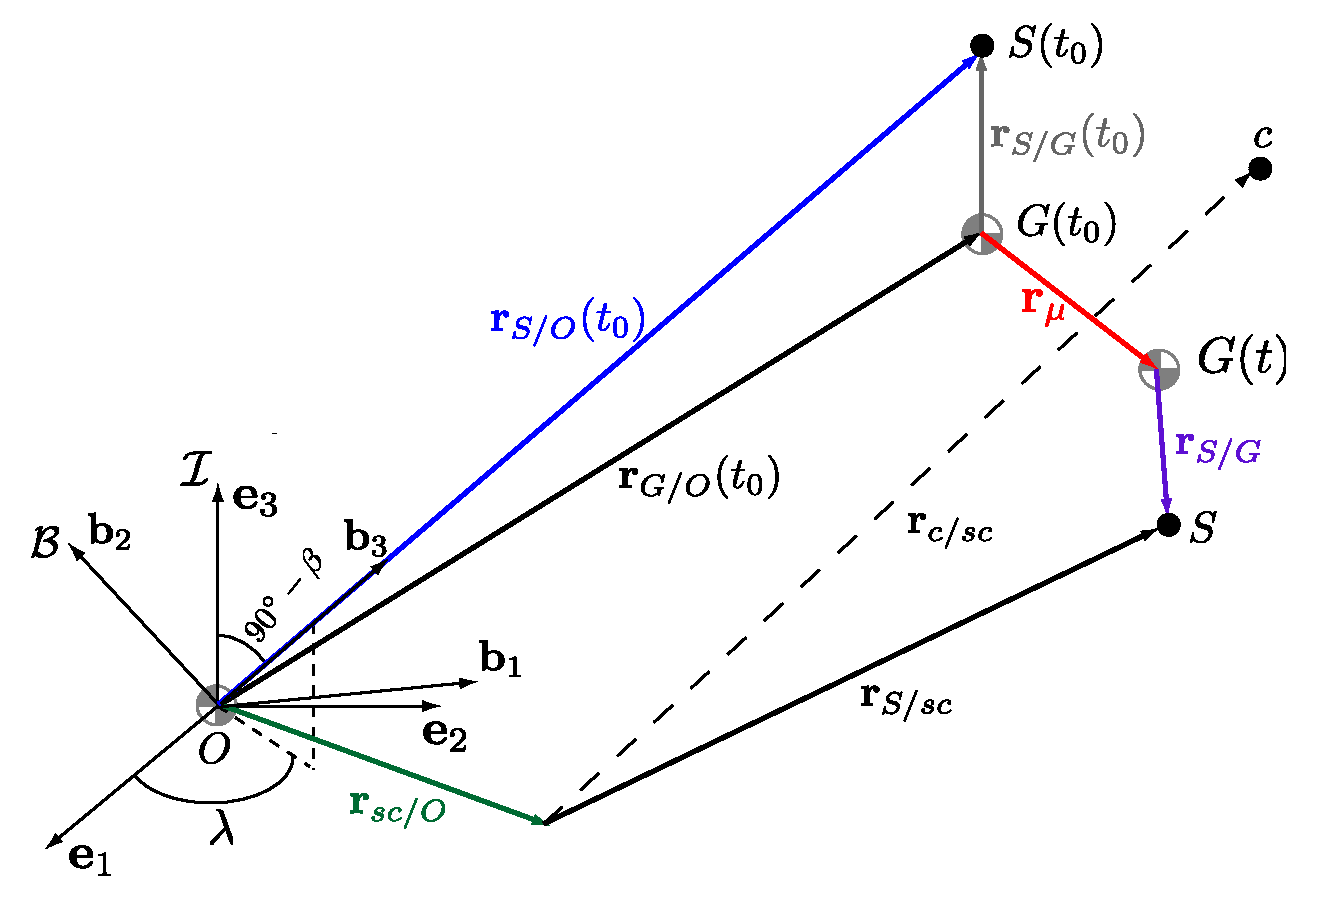
\includegraphics[width=6in]{./figures/ast_model}
 \caption[Astrometric observation schematic]{ A schematic of an astrometric observation.  The solar system barycenter is placed at the origin of frame $\mathcal{I}$, while the observed star system's barycenter at epoch $t_0$ is at $G(t_0)$ and at $G(t)$ at observation time $t$.  $S$ represents the star position at time $t$ and point $c$ represents the (possibly time-varying) position of the centroid of a group of reference stars.}
\label{fig:ast_model} 
\end{figure} 

Figure \ref{fig:ast_model} defines the vectors and reference frames used to describe an astrometric observation of an exosystem.
Reference frame $\mathcal{I}$ is the inertially fixed, barycentric/ ecliptic frame located at the solar system barycenter with the unit vector $\mathbf{e}_3$ directed perpendicular to the ecliptic plane (the $\mathbf{e}_1$ and $\mathbf{e}_2$ unit vectors are arbitrary).  We define a second inertially fixed frame, called the tangent frame, $\mathcal{B}\addsymbol{$\mc B$}{Tangent frame}$, with $\mathbf{b}_3$ axis aligned with $\hat{\R}_{S/O}(t_0)$, the unit vector to the star at the reference time $t_0$.  The $\mathbf{b}_1$ axis is perpendicular to the plane containing $\R_{S/O}(t_0)$ and $\mathbf{e}_3$.  The final unit vector direction, $\mathbf{b}_2$, is mutually perpendicular to $\bc_1$ and $\R_{S/O}(t_0)$.
Given these definitions, we can express the three unit vectors defining $\mathcal{B}$ using coordinates in $\mathcal{I}$ as:
%
\begin{eqnarray}
\hat{\R}_{S/O}(t_0) \equiv \bc_3 &=&  \left[ \begin{array}{ccc} \cos \lambda \cos \beta &\sin \lambda \cos \beta & \sin \beta \end{array}\right]^T_\mathcal{I} \label{eq:rhat_0def} \nonumber\\
\bc_1 &=& \left[ \begin{array}{ccc} 0 & 0 & 1\end{array}\right]^T_\mathcal{I} \times \frac{\hat{\R}_s(t_0)}{\cos\beta} =  \left[ \begin{array}{ccc} -\sin \lambda &\cos \lambda & 0 \end{array}\right]^T_\mathcal{I} \\
\bc_2 &=& \hat{\R}_{S/O}(t_0) \times \bc_1  = \left[ \begin{array}{ccc} -\cos \lambda \sin \beta &-\sin \lambda \sin \beta& \cos \beta \end{array}\right]^T_\mathcal{I} \nonumber
\end{eqnarray}
%
where $\hat\R_{S/O}(t_0)$ is the unit vector to the star as given by its ecliptic coordinates at epoch $t_0$: $(\lambda,\beta)$, measured in the $\mathcal I$ frame.  This definition of frames assumes constant relative velocities between exosystem and local barycenters (i.e., constant proper motions).  For the time scales on which astrometric observations are taken, this is reasonable, but this derivation may have to be expanded if dealing with an accelerating exosystem.

We define the parallax by the small quantity:
\begin{equation}\label{eq:parallaxdef}
\varpi \triangleq \frac{a_0}{\Vert \R_{S/O}(t_0) \Vert} \,,
\end{equation}
where $a_0$ is a distance constant such that $\varpi\addsymbol{$\varpi$}{Parallax}$ is in units of radians.  Thus, $\R_{S/O}(t_0) = (a/\varpi) \hat\R_{S/O}(t_0)$ for $a_0 = 1$ AU, with $\R_s(t_0)$ expressed in AU.  An estimate of $\varpi$ provides the distance to the target star at epoch $t_0$.  The motion of the barycenter of the target star system, $\R_\mu$, is considered as motion in the tangent reference frame,
\begin{equation}\addsymbol{$\R_\mu$}{Exosystem barycenter motion vector}
\R_\mu(t) = \sigma_x (t - t_0) \bc_1 + \sigma_y (t - t_0) \bc_2 + \sigma_z (t - t_0) \hat\R_s(t_0) \,,
\end{equation}
where $\sigma_i$ are the components of barycenter velocity at epoch $t_0$.  We approximate this velocity to be constant, as is usually done when considering short time spans such as  a space-based observatory's lifetime.  This expression is generally split into two components: the transverse and radial velocities.  Following \citet{green1985spherical}, we can write:
\begin{equation}\label{eq:veldef}
\begin{split}
\fddt{I} \R_{G/O}(t) &\equiv  \fddt{I} \left(\R_{G/O}(t_0) + \R_\mu(t)\right) =\fddt{I}\R_\mu(t)\\
  &= V_R  \hat\R_{S/O}(t_0) + \mathbf{V}_T \\
  \textrm{where} \quad  \mathbf{V}_T  &= \hat \R_{S/O}(t_0) \times \left(\fddt{I} \R_{G/O}(t) \times \hat \R_{S/O}(t_0)\right) \, .
 \end{split}
\end{equation}

In our notation, $V_R\addsymbol{$V_R$}{Radial velocity}$ is just $\sigma_z$, whereas $\mathbf{V}_T\addsymbol{$\mathbf{V}_T$}{Transverse velocity}$ is the vector $\left[\begin{matrix} \sigma_x & \sigma_y & 0 \end{matrix}\right]^T$.  The transverse velocity (multiplied by time) thus gives the proper motion of the barycenter (motion in the plane of the sky), which has the largest effect on the position of the target system at the time of observation.  However, the radial velocity also has a measurable effect on the astrometric observation.  Because motion of the target system in the radial direction causes the distance to the system to change, we observe a difference in the direction to the target star, known as `perspective acceleration'.  The third component of $\R_\mu$ (and thus $\sigma_z$) interacts in non-negligible ways with other values in the measurement, and is thus observable.  However, when dealing with \emph{a priori} estimates of these velocity components  it is important to note that the transverse and radial velocities are measured in different ways (i.e., astrometry vs.~doppler spectroscopy).  We will also find it convenient to have an expression for the normalized barycenter motion,
\begin{equation}
\bar{\R}_\mu \triangleq \frac{\R_\mu}{\|\R_{S/O}(t_0)\|} = \bar \sigma_x (t - t_0) \bc_1 + \bar\sigma_y (t - t_0) \bc_2 + \bar\sigma_z (t - t_0) \hat\R_{S/O}(t_0) \,,
\end{equation}
where $\bar\sigma_x$, $\bar\sigma_y$, and $\bar\sigma_z$ are the nondimensional barycenter velocities in radians/time unit.

Finally, we must consider what exactly is measured during an astrometric observation.  While we will focus on astrometric methods that employ interferometers, it is important to note that there are other astrometric instrument designs.  All of these, however, make some measurement of the observer-target star unit vector, and so the analysis above is fully applicable.  An interferometer, in particular, measures the projection of a target direction onto the instrument's baseline vector, recorded as the optical path-length delay (OPD)$\addsymbol{OPD}{Optical path delay}$ between the two interferometer detectors:
\begin{equation}
\textrm{OPD} = \mf B \cdot \hat{\mf r}_{S/sc}  + k + n \,,
\end{equation}
where $\mf B\addsymbol{$\mf B$}{Observatory orientation vector}$ is the orientation vector of an interferometer of baseline length $B = \Vert \mf B \Vert$, $k$ is a constant term representing the offset of the optical path differences, and $n$ is the measurement noise.
Planet-finding is generally proposed in a narrow angle mode, where the measurement is the relative OPD between two sources in a field of view, performed in quick succession such that $k$ remains nearly constant, and is assumed to cancel in subtraction.  Typically each target star has multiple reference sources, so the combined differential OPD ($\Delta$OPD) is with respect to a centroid position.  The measurement is also repeated for two (preferably orthogonal) interferometer baseline orientations to track the 2D position of the target in the plane of the sky.  Assuming that the interferometer baselines are taken as directions $\mf b_1$ and $\mf b_2$ of our body frame, then the astrometric measurement becomes:
\begin{equation}\label{eq:measurement}
\mf d = B\left[ \begin{array}{l} \mf b_1 \cdot \left(\hat{\mf r}_{S/sc} - \hat{\mf r}_{c/sc}\right) \\\mf b_2 \cdot \left(\hat{\mf r}_{S/sc} - \hat{\mf r}_{c/sc}\right) \end{array}\right] + \mf n \,,
\end{equation}
where $B$ is the size of the interferometer baseline and $\mf n$ is an additive noise vector due to measurement error.  

In the literature, the measurement in \refeq{eq:measurement} is often described as the angular separation between the two sources, projected onto the baseline \citep{konacki2002frequency,sozzetti2002,sozzetti2003}; it is assumed that $\mf d$ scaled by $B$ is a radian measure that can be converted to other angular units such as arcseconds.  It is this assumption that leads to the terminology of $\mu$as-precise astrometry, as the required sensitivity of the instrument to changes in the OPDs, when treated as an angle, evaluates to under 1 $\mu$as.  

In fact, \citet{colavita1994measurement} points out that, using the definition for $\hat{\mf r}_{S/sc}$ in \refeq{eq:rhat_0def}, for a centroid separation of ($\Delta \lambda$, $\Delta \beta$), the difference in unit vectors, to first order, can be written as,
\begin{equation}\label{eq:sdiff_fo}
\hat{\mf r}_{S/sc} - \hat{\mf r}_{c/sc} \approx \left[\begin{matrix} 
\sin\beta\cos\lambda\Delta\beta + \cos\beta\sin\lambda\Delta\lambda\\
\sin\beta\sin\lambda\Delta\beta - \cos\beta\cos\lambda\Delta\lambda\\
-\cos\beta\Delta\beta \end{matrix}\right]_\mathcal{I} \, .
\end{equation}
In this way, knowledge of the baseline vector and the differential OPD allows you to calculate a vector which maps in a relatively simple fashion (to first order) to two spherical angles representing the separation between the target and centroid.

\begin{figure}[ht]
\centering
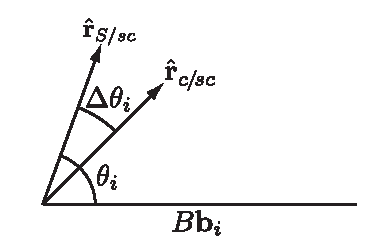
\includegraphics[width=2.75in]{./figures/narrow_angle_model}
 \caption[Narrow angle astrometry schematic]{ A schematic of a narrow-angle astrometric measurement.  $B$ is the size of the interferometer baseline.}
\label{fig:narrow_mode_model} 
\end{figure} 

Unfortunately, such a direct first order mapping between \refeq{eq:measurement} and the angle between the target and centroid is not very accurate.  An OPD has units of distance or time (with the converting factor equal to the speed of light), and so a differential OPD will also have values equal to fractions of the interferometer baseline.  Let us assume that the (flat) wavefront from the target star is incident on the interferometer baseline with angle $\theta_i$, and that the centroid is located at an angle $\Delta\theta_i$ from the target star, in the projection of the sky due to interferometer orientation $\mf b_i$ (Figure \ref{fig:narrow_mode_model} --- $\Delta\theta_i$ is analogous to $\Delta\lambda$ and $\Delta\beta$ in \refeq{eq:sdiff_fo}).
The components of the measurement (without the noise term) are then,
\begin{equation}
d_i =B \left(\cos\theta_i - \cos(\theta_i - \Delta\theta_i)\right) =B\left(\cos\theta_i(1 - \cos\Delta\theta_i) - \sin\theta_i \sin\Delta\theta_i\right) \,.
\end{equation}

We are primarily interested in changes in the angle $\Delta\theta_i$, since this determines the movement of the target star with respect to the centroid in time (of course, this is further complicated by possible motion of the centroid itself).  Assuming this to be a small angle, we can substitute the Taylor series expansions of the sine and cosine terms in $\Delta\theta_i$ to first order to find,
\begin{equation}
d_i \approx -B \sin\theta_i \Delta\theta_i \, .
\end{equation}
Thus, by scaling the differential OPD by the interferometer baseline length and the direction on the sky of the target ($B\sin\theta_i$), we do get a first order approximation of the angular difference between the target and centroid (assuming perfect a priori knowledge of the target's (or equivalently centroid's) location with respect to the interferometer orientation).  Unfortunately, if we assume the target star to be on the order of 1$^\circ$ from the centroid \citep{sozzetti2002,shao1992potential}, the first of the dropped terms ($\Delta\theta_i^2/2$) has a magnitude of 1.5$\times10^{-4}$ rad, or 31.4 arcseconds.  When discussing ultra-precise applications, it is therefore inaccurate to treat the values produced by \refeq{eq:measurement} as directly mapping to angular measures.  For these reasons, we treat all derived values as dimensionless for the remainder of this discussion, normalizing all distances and converting all angles to radians to remain consistent.  It is also important to point out that in this discussion, we consistently assume zero pointing error.  For a real instrument, accurate knowledge of the baseline vectors will be built up over many individual observations, each with an associated measurement error, but neither the interferometer orientation, nor the exact length of the baseline, can ever be known with perfect precision.  In order to include a pointing and baseline length error, we would need to extend the measurement equation, and update all subsequent calculations.

With these definitions and considerations, we can write the exact astrometric measurement  in terms of known quantities and the quantities whose values we wish to determine.  This is done by writing the vector from the spacecraft to the target star, $\mf r_{S/sc}$, in terms of the initial reference vector, $\R_{S/O}(t_0)$,
%
\begin{eqnarray}
\R_{S/sc} & = & \R_{S/O}(t_0) - \R_{S/G}(t_0) + \R_\mu + \R_{S/G} - \R_{sc/O} \nonumber \\
& = & \R_{S/O}(t_0) + \R_\mu + \Delta \R_{S/G} - \R_{sc/O} \,,
\end{eqnarray}
where $\R_{sc/O}$ is the spacecraft position vector relative to the solar system barycenter and  $\Delta \R_{S/G}$ is the difference in the star's position relative to $G$ between $t_0$ and epoch. We can then find the unit vector in the direction of $\R_{S/sc}$,
%
\begin{equation}\label{eq:rhat_ssc}
\begin{split}
\hat\R_{S/sc} &= \frac{\R_{S/sc}}{\| \R_{S/sc} \|}  \\
&= (\R_{S/O}(t_0) + \R_\mu +\Delta \R_{S/G}- \R_{sc/O})\times  \\
&\hspace{3ex}  \left\{\R_{S/O}(t_0)\cdot\R_{S/O}(t_0) + \R_\mu \cdot \R_\mu + \Delta \R_{S/G} \cdot \Delta \R_{S/G} +\R_{sc/O} \cdot \R_{sc} \right. \\
&\hspace{3.5ex}{}+ 2\R_{S/O}(t_0) \cdot \R_\mu + 2\R_{S/O}(t_0) \cdot \Delta \R_{S/G} - 2\R_{S/O}(t_0) \cdot \R_{sc/O} \\
&\hspace{3.5ex}\left.{} + 2 \R_\mu \cdot \Delta \R_{S/G} - 2 \R_\mu \cdot \R_{sc/O} - 2 \Delta \R_{S/G} \cdot \R_{sc/O}\right\}^{-\frac{1}{2}} \,. 
 \end{split}
\end{equation}

The spacecraft to centroid pointing unit vector, $\hat{\mf r}_{c/sc}$, can be similarly expressed by using \refeq{eq:rhat_ssc} for each reference source with the appropriate values for $\R_{S/O}(t_0)$ and $\R_\mu$.  When using this model for the reference sources, it is important to note that for a source $n$, $\hat\R_{n}(t_0)$ is not aligned with $\hat\R_{S/O}(t_0)$ and is thus not orthogonal to $\mf b_1$ and $\mf b_2$.  When evaluating \refeq{eq:measurement}, this simply means that all vectors have to be expressed as components in the same reference frame, which requires a change of coordinates for the reference sources.  If we assume extragalactic references with no companions or planets, the variation in the centroid position will be many orders of magnitudes below our desired level of accuracy.  Unfortunately, such references are not always available, and so these effects may become significant if one or more of the references is within our galaxy and has companions of its own.

\subsection{Doppler Spectroscopy Observables and Constraints}\label{sec:rv_inst_obs}
Unlike astrometry, which uses interferometers to find the instantaneous position of the star in the plane of the sky, doppler spectroscopy utilizes high-resolution spectrometers to measure the instantaneous velocity of the star along the line of sight.  Calibration sources such as cathode lamps and absorption cells are used to produce highly accurate spectra \citep{vogt1994hires}.  Following \citet{marcy1992precision} and \citet{butler1996attaining}, we model the observation as starlight passing through an absorption cell (e.g., iodine), which creates a combined spectrum of absorption bands from the star's spectrum and the cell.  This combined spectrum is passed through an echelle spectrometer \citep{vogt1987lick} and dispersed onto the detector as a nearly linear function in wavelength.

Any shift in the stellar spectrum must be modeled as due to Doppler effects and instrumental effects including mechanical instabilities, thermal effects, and the alignment of the optical system.  The observed spectrum can then be written as:
\begin{equation}\label{eq:obsSpectrum}
I_{obs}(\lambda) = \kappa \left[ I_S(\lambda + \Delta\lambda_S)T_C(\lambda + \Delta\lambda_C) \right] \otimes \PSF
\end{equation}
where $I_S$ is the stellar spectrum, $\Delta\lambda_S$ is the shift of the stellar spectrum, $T_C$ is the transmission function of the absorption cell, and $\Delta\lambda_C$ is the shift of the transmission function. The constant $\kappa$ is directly proportional to the integration time of the observation.  The transmission function is measured directly with the use of another spectrometer (for example a Fourier Transform Spectrometer \citep{davis2001fourier}), while the stellar spectrum may be derived from high signal-to-noise observations of the target star by means of PSF deconvolution \citep{gilliland1992resolution}.  The remaining parameters are determined by fitting the observed spectrum to \refeq{eq:obsSpectrum}.

The Doppler shift is parameterized as $\Delta\lambda/\lambda$, where:
\begin{equation}
\Delta\lambda \triangleq \Delta\lambda_S - \Delta\lambda_C \,.
\end{equation}
This can be related to the star's velocity via the relativistic Doppler equation:
\begin{equation}\label{eq:doppler}
\frac{\Delta\lambda}{\lambda} = \frac{\left(1 + \left(\frac{v}{c}\right)^2\cos\theta\right)\left(1 + \rho_g\right)}{n\sqrt{1 - \left(\frac{v}{c}\right)^2}} - 1
\end{equation}
where $n$ is the index of refraction of the air column over the spectrograph and  $\rho_g$ is the gravitational redshift of the starlight.  The velocity $v$ is defined as the magnitude of the velocity of the target star with respect to the observer ($v = \Vert \leftexp{\mc I}{\mf v_{S/sc}}\Vert$) while $\theta$ is the angle between the line of sight and the star's velocity vector:
\begin{equation}
\cos\theta = \hat{\mf r}_{S/sc}\cdot \leftexp{\mc I}{\hat{\mf v}_{S/sc}} \,.
\end{equation}

If we take $\theta = 0$ \refeq{eq:doppler} becomes:
\begin{equation}
\frac{\Delta\lambda}{\lambda} = \frac{\left(1 + \rho_g\right)}{n} \sqrt{\frac{\left(1 + \frac{v}{c}\right)}{1 -\frac{v}{c}}} - 1 \,.
\end{equation}
If $v \ll c$, the Taylor expansion of this expression gives us:
\begin{equation}
\frac{\Delta\lambda}{\lambda} = \frac{\left(1 + \rho_g\right)}{n}\left(1 + \frac{v}{c} + \mc O\left( \left(\frac{v}{c}\right)^2\right) - 1\right) \approx \frac{v}{c} \,.
\end{equation}
We thus have an approximate linear mapping of the doppler spectroscopy observables to the star's line of sight velocity.  Current ground-based observations have precisions of order 1 m s$^{-1}$ \citep{butler2006}, although improvements in instrumentation and calibration may provide us with precisions of order 1 cm s$^{-1}$ in the near future \citep{lovis2006exoplanet}.  Together with the astrometric measurement, doppler spectroscopy provides a third spatial component, making the full three-dimensional orbit observable, given that sufficient measurement accuracy is achieved.


\section{Transit Photometry}\label{sec:photometry}

Of all of the methods so far discussed, transit photometry has the largest resource requirements as it demands constant monitoring of the target star.  It also represents the least likely event, since the orientation of the orbit has to be such that the planet will obscure the star at some point, from the point of view of the observer.

\begin{figure}[ht]
\centering
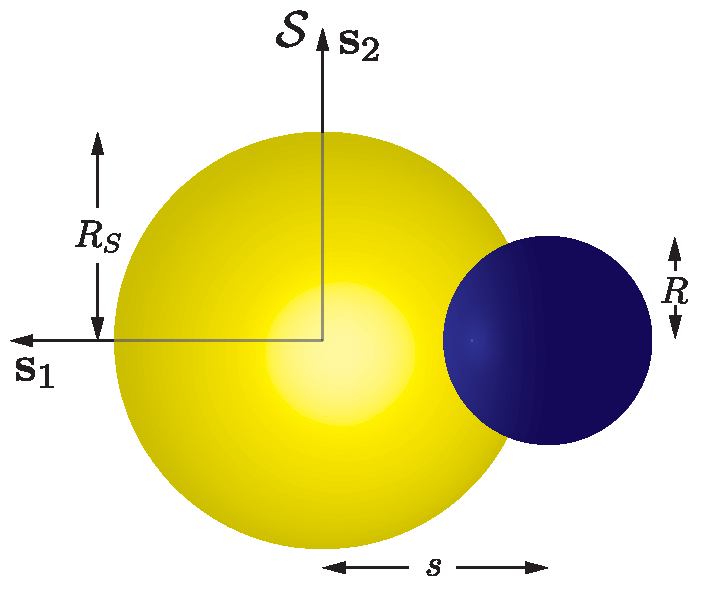
\includegraphics[width=4in]{./figures/phot_model}
 \caption[Transit schematic]{ A schematic of a photometric transit observation.  The amount of starlight occluded from the observer's point of view is determined by the star and planet radii ($R_S$ and $R$) and the apparent separation $s$.}
\label{fig:phot_model} 
\end{figure} 

\reffig{fig:phot_model} presents a schematic view of a transit in the plane of the sky.  The amount of starlight occluded can be expressed as a function of the star and planet radii and the apparent separation.  Following \citet{mandel2002analytic}, we can express the ratio of obscured ($F^{(e)}_S\addsymbol{$F^{(e)}_S$}{Obscured stellar flux}$) to unobscured starlight, assuming a uniform source and an opaque eclipsing body, as:

\begin{equation} \label{eq:transitFe}
 \frac{F^{(e)}_S}{F_S} = 
\left\{ \begin{array}{l l}
1 & R_S + R < s\\
1 - \frac{1}{\pi} \left[ \frac{R^2 }{R_S^2}\kappa_0 + \kappa_1 - \sqrt{\frac{s^2}{R_S^2} - \frac{\left( R_S^2 + s^2 - R^2\right)^2}{4 R_S^4}}\right] & \vert R_S - R \vert < s \le R_S + R \\
1 - \left(\frac{R}{R_S}\right)^2 & s \le R_S - R\\
0 & s \le R - R_S
\end{array} \right. 
\end{equation}
where
\begin{equation}
\kappa_0 = \cos^{-1}\left(\frac{R^2 +s^2 - R_S^2}{2Rs}\right) \quad\textrm{and}\quad \kappa_1 =  \cos^{-1}\left(\frac{R_S^2 - R^2 + s^2}{2R_S s}\right)
\end{equation}
where $R_S\addsymbol{$R_S$}{Star radius}$ is the stellar radius.

These equations allow us to model the `dip' in the photometric output of an exosystem associated with a transiting exoplanet, but there are many additional photometric effects that can be observed.  Stars are not perfectly uniform sources, which produces limb darkening and  causes more significant dimming during eclipse \citep{mandel2002analytic,claret2008testing}.  Furthermore, effects due to atmospheric lensing and projected oblateness can be inferred from sufficiently precise transit photometry \citep{hui2002atmospheric}.  While all of these can improve our modeling of exosystems, they will not be explicitly considered in this thesis.  However, as these effects may be modeled using the same parameter set employed throughout this chapter, they may be simulated and analyzed using the same methods that will be introduced in Chapters \ref{ch:param_dists} and \ref{ch:obs_sims}.

